% Created 2011-10-03 Mon 12:55
\documentclass[captions=tableheading]{scrbook}


%%%%%%%%%%%%%%%%%%%%%%%%%%%%%% User specified LaTeX commands.
% Meta information - fill between {} and do not remove %
% \VignetteIndexEntry{An Introduction to Probability and Statistics Using R}
% \VignetteDepends{}
% \VignetteKeywords{}
% \VignettePackage{IPSUR}
% Package

\usepackage{lmodern}
\renewcommand{\sfdefault}{lmss}
\renewcommand{\ttdefault}{lmtt}

% needed packages
\usepackage{amsmath}
\usepackage{amssymb}
\usepackage{amsthm}
\usepackage{babel}
\usepackage{epsfig}
\usepackage{fixltx2e}
\usepackage{float}
%\usepackage{floatflt}
\usepackage[T1]{fontenc}
\usepackage{footnote}
\usepackage{graphics}
\usepackage{graphicx}
\usepackage[utf8]{inputenc}
\usepackage{latexsym}
\usepackage{longtable}
\usepackage{makeidx}
\usepackage{marvosym}
\usepackage{multicol}
%\usepackage{pslatex}
\usepackage{rotating}
%\usepackage{showidx}
\usepackage{soul}
\usepackage{srcltx}
\usepackage{stmaryrd}
\usepackage{subfig}
\usepackage{textcomp}
%\usepackage{theorem}
\usepackage[subfigure]{tocloft}
\usepackage{txfonts}
\usepackage{upgreek}
\usepackage{url}
\usepackage{varioref}
\usepackage{verbatim}
\usepackage{wasysym}
\usepackage{wrapfig}


% Page setup
\usepackage[paperwidth=7.44in,paperheight=9.69in]{geometry}
\geometry{verbose,tmargin=1in,bmargin=1in,lmargin=1in,rmargin=1in}
\pagestyle{headings}
\setcounter{secnumdepth}{2}
\setcounter{tocdepth}{1}

\makeindex

% PDF settings
\usepackage[hyperref,x11names]{xcolor}
\usepackage[	unicode=true, 
		bookmarks=true, 
		bookmarksnumbered=true, 
		bookmarksopen=true, 
		bookmarksopenlevel=0, 
		breaklinks=true,
		pdfborder={0 0 0},
		backref=page,
		colorlinks=true]{hyperref}
\hypersetup{pdftitle={Introduction to Probability and Statistics Using R},
 		pdfauthor={G. Jay Kerns}, 
		linkcolor=Firebrick4, 
		citecolor=black, 
		urlcolor=SteelBlue4}

% Listings setup
\usepackage{color}
\usepackage{listings}
\lstset{basicstyle={\ttfamily},
	language=R,
	breaklines=true,
	breakatwhitespace=true,
	keywordstyle={\ttfamily},
	numberstyle = {\ttfamily},
	morestring=[b]"
}




%%%%%%%%%%%%%%%%%%%%%%%%%%%%%% LyX specific LaTeX commands.
\providecommand{\LyX}{L\kern-.1667em\lower.25em\hbox{Y}\kern-.125emX\@}
\newcommand{\noun}[1]{\textsc{#1}}
%% Because html converters don't know tabularnewline
\providecommand{\tabularnewline}{\\}

% special logos
\providecommand{\IPSUR}
{\textsc{I\kern 0ex\lower-.3ex\hbox{\small P}\kern -.5ex\lower.4ex\hbox{\footnotesize S}\kern -.25exU}\kern -.1ex\lower .15ex\hbox{\textsf{\large R}}\@}

\providecommand{\IPSURtitle}
{\fontsize{30}{35}\selectfont \textsc{I\kern -.16ex\lower-.5ex\hbox{\Large P}\kern -.5ex\lower.4ex\hbox{\Large S}\kern -.25exU}\kern -.1ex\lower .15ex\hbox{\textsf{\Huge R}}\@}


%  user defined commands
% special operators
\renewcommand{\P}{\mathrm{I\hspace{-1.5pt}P}}
\newcommand{\E}{\mathrm{I\hspace{-1.5pt}E}}
\renewcommand{\vec}[1]{\mbox{\boldmath$#1$}}

% special symbols
\newcommand{\me}{\mathrm{e}}
\newcommand{\R}{\mathbb{R}}
\newcommand{\diff}{\mathrm{d}}
\newcommand{\ybar}{\overline{y}}
\newcommand{\xbar}{\overline{x}}
\newcommand{\Xbar}{\overline{X}}
\newcommand{\Ybar}{\overline{Y}}


\makeatletter


%%%%%%%%%%%%%%%%%%%%%%%%%%%%%% Textclass specific LaTeX commands.
\newcommand{\Rcode}[1]{{\texttt{#1}}}
\newcommand{\Robject}[1]{{\texttt{#1}}}
\newcommand{\Rcommand}[1]{{\texttt{#1}}}
\newcommand{\Rfunction}[1]{{\texttt{#1}}}
\newcommand{\Rfunarg}[1]{{\textit{#1}}}
\newcommand{\Rpackage}[1]{{\textit{#1}}}
\newcommand{\Rmethod}[1]{{\textit{#1}}}
\newcommand{\Rclass}[1]{{\textit{#1}}}
\numberwithin{equation}{section}
\numberwithin{figure}{section}
\theoremstyle{plain}
\ifx\thechapter\undefined
\newtheorem{thm}{Theorem}
\else
\newtheorem{thm}{Theorem}[chapter]
\fi
 \theoremstyle{definition}
  \newtheorem{example}[thm]{Example}
  \theoremstyle{plain}
  \newtheorem{fact}[thm]{Fact}
\newenvironment{lyxcode}
{\par\begin{list}{}{
\setlength{\rightmargin}{\leftmargin}
\setlength{\listparindent}{0pt}% needed for AMS classes
\raggedright
\setlength{\itemsep}{0pt}
\setlength{\parsep}{0pt}
\normalfont\ttfamily}%
 \item[]}
{\end{list}}
  \theoremstyle{definition}
  \newtheorem{xca}[thm]{Exercise}
  \theoremstyle{remark}
  \newtheorem{note}[thm]{Note}
  \theoremstyle{plain}
  \newtheorem{ax}[thm]{Axiom}
  \theoremstyle{plain}
  \newtheorem{prop}[thm]{Proposition}
  \theoremstyle{definition}
  \newtheorem{defn}[thm]{Definition}
  \theoremstyle{remark}
  \newtheorem{rem}[thm]{Remark}
  \theoremstyle{plain}
  \newtheorem{cor}[thm]{Corollary}
  \theoremstyle{plain}
  \newtheorem{assumption}[thm]{Assumption}
  \theoremstyle{remark}
  \newtheorem*{note*}{Note}

\setlength{\cftfignumwidth}{1.5cm}

\@ifundefined{showcaptionsetup}{}{%
 \PassOptionsToPackage{caption=false}{subfig}}
\usepackage{subfig}
\AtBeginDocument{
  \def\labelitemii{\(\circ\)}
}

\makeatother





\providecommand{\alert}[1]{\textbf{#1}}

\title{Introduction to Probability and Statistics Using R}
\author{G. Jay Kerns}
\date{\today}

\begin{document}

\maketitle

% Org-mode is exporting headings to 2 levels.


\pagenumbering{roman}
\setcounter{page}{2}

\noindent \IPSUR: Introduction to Probability and Statistics Using \textsf{R}

\noindent Copyright \textcopyright~2011 G.~Jay Kerns
\noindent ISBN: 978-0-557-24979-4
\medskip{}


\noindent Permission is granted to copy, distribute and/or modify
this document under the terms of the GNU Free Documentation License,
Version 1.3 or any later version published by the Free Software Foundation; with no Invariant Sections, no Front-Cover Texts, and no Back-Cover Texts. A copy of the license is included in the section entitled ``GNU Free Documentation License''.

\vspace{0.5in}
\noindent Date: \today
\noindent \vfill{}

\cleardoublepage
\phantomsection
\pdfbookmark[1]{Contents}{table}

\tableofcontents{}




\cleardoublepage
\phantomsection
\addcontentsline{toc}{chapter}{Preface to the Second Edition}

\chapter*{Preface to the Second Edition}

What is new in the Second Edition?  Almost everything.  I have addressed two of the goals from the first edition.  I have now converted most of the plots to \texttt{ggplot2} format. 

%    IPSUR: Introduction to Probability and Statistics Using R
%    Copyright (C)  2013 G. Jay Kerns
%
%    This file is part of IPSUR.
%
%    Permission is granted to copy, distribute and/or modify this document
%    under the terms of the GNU Free Documentation License, Version 1.3
%    or any later version published by the Free Software Foundation;
%    with no Invariant Sections, no Front-Cover Texts, and no Back-Cover Texts.
%    A copy of the license is contained in the LICENSE file in this 
%    directory.


\cleardoublepage
\phantomsection
\addcontentsline{toc}{chapter}{Preface to the First Edition}

\chapter*{Preface to the First Edition}

This book was expanded from lecture materials I use in a one semester upper-division undergraduate course entitled \emph{Probability and Statistics} at Youngstown State University. Those lecture materials, in turn, were based on notes that I transcribed as a graduate student at Bowling Green State University. The course for which the materials were written is 50-50 Probability and Statistics, and the attendees include mathematics, engineering, and computer science majors (among others). The catalog prerequisites for the course are a full year of calculus.

The book can be subdivided into three basic parts. The first part includes the introductions and elementary \emph{descriptive statistics}; I want the students to be knee-deep in data right out of the gate. The second part is the study of \emph{probability}, which begins at the basics of sets and the equally likely model, journeys past discrete/continuous  random variables, and continues through to multivariate distributions. The chapter on sampling distributions paves the way to the third part, which is \emph{inferential statistics}. This last part includes point and interval estimation, hypothesis testing, and finishes with introductions to selected topics in applied statistics.

I usually only have time in one semester to cover a small subset of this book. I cover the material in Chapter 2 in a class period that is supplemented by a take-home assignment for the students. I spend a lot of time on Data Description, Probability, Discrete, and Continuous Distributions. I mention selected facts from Multivariate Distributions in passing, and discuss the meaty parts of Sampling Distributions before moving right along to Estimation (which is another chapter I dwell on considerably). Hypothesis Testing goes faster after all of the previous work, and by that time the end of the semester is in sight. I normally choose one or two final chapters (sometimes three) from the remaining to survey, and regret at the end that I did not have the chance to cover more.

In an attempt to be correct I have included material in this book which I would normally not mention during the course of a standard lecture. For instance, I normally do not highlight the intricacies of measure theory or integrability conditions when speaking to the class. Moreover, I often stray from the matrix approach to multiple linear regression because many of my students have not yet been formally trained in linear algebra. That being said, it is important to me for the students to hold something in their hands which acknowledges the world of mathematics and statistics beyond the classroom, and which may be useful to them for many semesters to come. It also mirrors my own experience as a student.

The vision for this document is a more or less self contained, essentially complete, correct, introductory textbook. There should be plenty of exercises for the student, with full solutions for some, and no solutions for others (so that the instructor may assign them for grading). By \texttt{Sweave}'s dynamic nature it is possible to write randomly generated exercises and I had planned to implement this idea already throughout the book. Alas, there are only 24 hours in a day. Look for more in future editions.

Seasoned readers will be able to detect my origins: \emph{Probability and Statistical Inference} by Hogg and Tanis \cite{Hogg2006}, \emph{Statistical Inference} by Casella and Berger \cite{Casella2002}, and \emph{Theory of Point Estimation} and \emph{Testing Statistical Hypotheses} by Lehmann \cite{Lehmann1998,Lehmann1986}. I highly recommend each of those books to every reader of this one. Some \(\mathsf{R}\) books with ``introductory'' in the title that I recommend are \emph{Introductory Statistics with R} by Dalgaard \cite{Dalgaard2008} and \emph{Using R for Introductory Statistics} by Verzani \cite{Verzani2005}. Surely there are many, many other good introductory books about \(\mathsf{R}\), but frankly, I have tried to steer clear of them for the past year or so to avoid any undue influence on my own writing.

I would like to make special mention of two other books: \emph{Introduction to Statistical Thought} by Michael Lavine \cite{Lavine2009} and \emph{Introduction to Probability} by Grinstead and Snell \cite{Grinstead1997}. Both of these books are \emph{free} and are what ultimately convinced me to release \IPSUR under a free license, too.

Please bear in mind that the title of this book is ``Introduction to Probability and Statistics Using \(\mathsf{R}\)'', and not ``Introduction to \(\mathsf{R}\) Using Probability and Statistics'', nor even ``Introduction to Probability and Statistics and \(\mathsf{R}\) Using Words''. The people at the party are Probability and Statistics; the handshake is \(\mathsf{R}\). There are several important topics about \(\mathsf{R}\) which some individuals will feel are underdeveloped, glossed over, or wantonly omitted. Some will feel the same way about the probabilistic and/or statistical content. Still others will just want to learn \(\mathsf{R}\) and skip all of the mathematics.

Despite any misgivings: here it is, warts and all. I humbly invite said individuals to take this book, with the GNU Free Documentation License (GNU-FDL) in hand, and make it better. In that spirit there are at least a few ways in my view in which this book could be improved.

\begin{description}
\item[Better data.] The data analyzed in this book are almost entirely from the \texttt{datasets} package in base \(\mathsf{R}\), and here is why:
\begin{itemize}
\item I made a conscious effort to minimize dependence on contributed packages,
\item The data are instantly available, already in the correct format, so we need not take time to manage them, and
\item The data are \emph{real}.
\end{itemize}
\end{description}

I made no attempt to choose data sets that would be interesting to the students; rather, data were chosen for their potential to convey a statistical point. Many of the data sets are decades old or more (for instance, the data used to introduce simple linear regression are the speeds and stopping distances of cars in the 1920's).

In a perfect world with infinite time I would research and contribute recent, \emph{real} data in a context crafted to engage the students in \emph{every} example. One day I hope to stumble over said time. In the meantime, I will add new data sets incrementally as time permits.
\begin{description}
\item[More proofs.] I would like to include more proofs for the sake of completeness (I understand that some people would not consider more proofs to be improvement). Many proofs have been skipped entirely, and I am not aware of any rhyme or reason to the current omissions. I will add more when I get a chance.
\item[More and better\~{}graphics.] I have not used the \texttt{ggplot2} package \cite{Wickam2009} because I do not know how to use it yet. It is on my to-do list.
\item[More and better exercises.] There are only a few exercises in the first edition simply because I have not had time to write more. I have toyed with the \texttt{exams} package \cite{exams} and I believe that it is a right way to move forward. As I learn more about what the package can do I would like to incorporate it into later editions of this book.
\end{description}


\section*{About This Document}
\IPSUR contains many interrelated parts: the \emph{Document}, the \emph{Program}, the \emph{Package}, and the \emph{Ancillaries}. In short, the \emph{Document} is what you are reading right now. The \emph{Program} provides an efficient means to modify the Document. The \emph{Package} is an \(\mathsf{R}\) package that houses the Program and the Document. Finally, the \emph{Ancillaries} are extra materials that reside in the Package and were produced by the Program to supplement use of the Document. We briefly describe each of them in turn.

\subsection*{The Document}

The \emph{Document} is that which you are reading right now -- \IPSUR's \emph{raison d'\^etre}. There are transparent copies (nonproprietary text files) and opaque copies (everything else). See the GNU-FDL in Appendix \ref{cha-GNU-Free-Documentation} for more precise language and details.

\begin{description}
\item[IPSUR.tex] is a transparent copy of the Document to be typeset with a \LaTeX{} distribution such as MikTeX or \TeX{} Live. Any reader is free to modify the Document and release the modified version in accordance with the provisions of the GNU-FDL. Note that this file cannot be used to generate a randomized copy of the Document. Indeed, in its released form it is only capable of typesetting the exact version of \IPSUR which you are currently reading. Furthermore, the \texttt{.tex} file is unable to generate any of the ancillary materials.
\item[IPSUR-xxx.eps, IPSUR-xxx.pdf] are the image files for every graph in the Document. These are needed when typesetting with \LaTeX{}.
\item[IPSUR.pdf] is an opaque copy of the Document. This is the file that instructors would likely want to distribute to students.
\item[IPSUR.dvi] is another opaque copy of the Document in a different file format.
\end{description}

\subsection*{The Program}

The \emph{Program} includes \texttt{IPSUR.lyx} and its nephew \texttt{IPSUR.Rnw}; the purpose of each is to give individuals a way to quickly customize the Document for their particular purpose(s).
\begin{description}
\item[IPSUR.lyx] is the source LyX file for the Program, released under the GNU General Public License (GNU GPL) Version 3. This file is opened, modified, and compiled with LyX, a sophisticated open-source document processor, and may be used (together with \texttt{Sweave}) to generate a randomized, modified copy of the Document with brand new data sets for some of the exercises and the solution manuals (in the Second Edition). Additionally, LyX can easily activate/deactivate entire blocks of the document, \emph{e.g.} the \emph{proofs} of the theorems, the student \emph{solutions} to the exercises, or the instructor \emph{answers} to the problems, so that the new author may choose which sections (s)he would like to include in the final Document (again, Second Edition). The \texttt{IPSUR.lyx} file is all that a person needs (in addition to a properly configured system) to generate/compile/export to all of the other formats described above and below, which includes the ancillary materials \texttt{IPSUR.Rdata} and \texttt{IPSUR.R}.
\item[IPSUR.Rnw] is another form of the source code for the Program, also released under the GNU GPL Version 3. It was produced by exporting \texttt{IPSUR.lyx} into \(\mathsf{R}\)/Sweave format (\texttt{.Rnw}). This file may be processed with Sweave to generate a randomized copy of \texttt{IPSUR.tex} -- a transparent copy of the Document -- together with the ancillary materials \texttt{IPSUR.Rdata} and \texttt{IPSUR.R}. Please note, however, that \texttt{IPSUR.Rnw} is just a simple text file which does not support many of the extra features that LyX offers such as WYSIWYM editing, instantly (de)activating branches of the manuscript, and more.
\end{description}

\subsection*{The Package}

There is a contributed package on \texttt{CRAN}, called \texttt{IPSUR}. The package affords many advantages, one being that it houses the  Document in an easy-to-access medium. Indeed, a student can have the Document at his/her fingertips with only three commands:



Another advantage goes hand in hand with the Program's license; since \IPSUR is free, the source code must be freely available to anyone that wants it. A package hosted on \texttt{CRAN} allows the author to obey the license by default.

A much more important advantage is that the excellent facilities at \(\mathsf{R}\)-Forge are building and checking the package daily against patched and development versions of the absolute latest pre-release of \(\mathsf{R}\). If any problems surface then I will know about it within 24 hours.

And finally, suppose there is some sort of problem. The package structure makes it \emph{incredibly} easy for me to distribute bug-fixes and corrected typographical errors. As an author I can make my corrections, upload them to the repository at \(\mathsf{R}\)-Forge, and they will be reflected \emph{worldwide} within hours. We aren't in Kansas anymore, Toto.

\subsection*{Ancillary Materials}

These are extra materials that accompany \IPSUR. They reside in the \texttt{/etc} subdirectory of the package source. 

\begin{description}
\item[IPSUR.RData] is a saved image of the \(\mathsf{R}\) workspace at the completion of the Sweave processing of \IPSUR. It can be loaded into memory with \texttt{File} \(\triangleright\) \texttt{Load Workspace} or with the command \texttt{load("/path/to/IPSUR.Rdata")}. Either method will make every single object in the file immediately available and in memory. In particular, the data BLANK from Exercise BLANK in Chapter BLANK on page BLANK will be loaded. Type BLANK at the command line (after loading \texttt{IPSUR.RData}) to see for yourself.
\item[IPSUR.R] is the exported \(\mathsf{R}\) code from \texttt{IPSUR.Rnw}. With this script, literally every \(\mathsf{R}\) command from the entirety of \IPSUR can be resubmitted at the command line.
\end{description}

\section*{Notation}

We use the notation \texttt{x} or \texttt{stem.leaf} notation to denote objects, functions, \emph{etc}.. The sequence \texttt{Statistics} \(\triangleright\) \texttt{Summaries} \(\triangleright\) \texttt{Active Dataset} means to click the \texttt{Statistics} menu item, next click the \texttt{Summaries} submenu item, and finally click \texttt{Active Dataset}.

\section*{Acknowledgements}

This book would not have been possible without the firm mathematical and statistical foundation provided by the professors at Bowling Green State University, including Drs. G\'{a}{}bor Sz\'{e}{}kely, Craig Zirbel, Arjun K. Gupta, Hanfeng Chen, Truc Nguyen, and James Albert. I would also like to thank Drs. Neal Carothers and Kit Chan. 

I would also like to thank my colleagues at Youngstown State University for their support. In particular, I would like to thank Dr. G. Andy Chang for showing me what it means to be a statistician.

I would like to thank Richard Heiberger for his insightful comments and improvements to several points and displays in the manuscript. 

Finally, and most importantly, I would like to thank my wife for her patience and understanding while I worked hours, days, months, and years on a \emph{free book}. Looking back, I can't believe I ever got away with it.

\vfill{}
\cleardoublepage
\phantomsection
\addcontentsline{toc}{chapter}{List of Figures}
\listoffigures

\vfill{}
\cleardoublepage
\phantomsection
\addcontentsline{toc}{chapter}{List of Tables}
\listoftables





\chapter{Continuous Distributions}
\label{sec-1}
\label{cha-Continuous-Distributions}


\noindent 
The focus of the last chapter was on random variables whose support can be written down in a list of values (finite or countably infinite), such as the number of successes in a sequence of Bernoulli trials. Now we move to random variables whose support is a whole range of values, say, an interval \((a,b)\). It is shown in later classes that it is impossible to write all of the numbers down in a list; there are simply too many of them.

This chapter begins with continuous random variables and the associated PDFs and CDFs The continuous uniform distribution is highlighted, along with the Gaussian, or normal, distribution. Some mathematical details pave the way for a catalogue of models.

The interested reader who would like to learn more about any of the assorted discrete distributions mentioned below should take a look at \emph{Continuous Univariate Distributions, Volumes 1} and \emph{2} by Johnson \emph{et al} \cite{Johnson1994,Johnson1995}.

\textbf{What do I want them to know?}
\begin{itemize}
\item how to choose a reasonable continuous model under a variety of physical circumstances
\item basic correspondence between continuous versus discrete random variables
\item the general tools of the trade for manipulation of continuous random variables, integration, \emph{etc}.
\item some details on a couple of continuous models, and exposure to a bunch of other ones
\item how to make new continuous random variables from old ones
\end{itemize}
\section{Continuous Random Variables}
\label{sec-1-1}
\label{sec-continuous-random-variables}
\subsection{Probability Density Functions}
\label{sec-1-1-1}
\label{sub-probability-density-functions}


Continuous random variables have supports that look like
\begin{equation}
S_{X}=[a,b]\mbox{ or }(a,b),
\end{equation}
or unions of intervals of the above form. Examples of random variables that are often taken to be continuous are:

\begin{itemize}
\item the height or weight of an individual,
\item other physical measurements such as the length or size of an object, and
\item durations of time (usually).
\end{itemize}

Every continuous random variable \(X\) has a \emph{probability density function} (PDF) denoted \(f_{X}\) associated with it
\footnote{Not true. There are pathological random variables with no density function. (This is one of the crazy things that can happen in the world of measure theory). But in this book we will not get even close to these anomalous beasts, and regardless it can be proved that the CDF always exists.}
that satisfies three basic properties:
\begin{enumerate}
\item \(f_{X}(x)>0\) for \(x\in S_{X}\),
\item \(\int_{x\in S_{X}}f_{X}(x)\,\mathrm{d} x=1\), and
\item \(\mathbb{P}(X\in A)=\int_{x\in A}f_{X}(x)\:\mathrm{d} x\), for an event \(A\subset S_{X}\).
\end{enumerate}

\begin{rem}
We can say the following about continuous random variables:
\begin{itemize}
\item Usually, the set \(A\) in \ref{enu-contrvcond3} takes the form of an interval, for example, \(A=[c,d]\), in which case
  \begin{equation}
  \mathbb{P}(X\in A)=\int_{c}^{d}f_{X}(x)\:\mathrm{d} x.
  \end{equation}
\item It follows that the probability that \(X\) falls in a given interval is simply the \emph{area under the curve} of \(f_{X}\) over the interval.
\item Since the area of a line \(x=c\) in the plane is zero, \(\mathbb{P}(X=c)=0\)  for any value \(c\). In other words, the chance that \(X\) equals a particular value \(c\) is zero, and this is true for any number \(c\). Moreover, when \(a<b\) all of the following probabilities are the same:
  \begin{equation}
  \mathbb{P}(a\leq X\leq b)=\mathbb{P}(a<X\leq b)=\mathbb{P}(a\leq X<b)=\mathbb{P}(a<X<b).
  \end{equation}
\item The PDF \(f_{X}\) can sometimes be greater than 1. This is in contrast to the discrete case; every nonzero value of a PMF is a probability which is restricted to lie in the interval \([0,1]\).
\end{itemize}

\end{rem}

We met the cumulative distribution function, \(F_{X}\), in Chapter \ref{cha-Discrete-Distributions}. Recall that it is defined by \(F_{X}(t)=\mathbb{P}(X\leq t)\), for \(-\infty<t<\infty\). While in the discrete case the CDF is unwieldy, in the continuous case the CDF has a relatively convenient form:
\begin{equation}
F_{X}(t)=\mathbb{P}(X\leq t)=\int_{-\infty}^{t}f_{X}(x)\:\mathrm{d} x,\quad-\infty<t<\infty.
\end{equation}

\begin{rem}
For any continuous CDF \(F_{X}\) the following are true.
\begin{itemize}
\item \(F_{X}\) is nondecreasing , that is, \(t_{1}\leq t_{2}\) implies \(F_{X}(t_{1})\leq F_{X}(t_{2})\).
\item \(F_{X}\) is continuous (see Appendix \ref{sec-Differential-and-Integral}). Note the distinction from the discrete case: CDFs of discrete random variables are not continuous, they are only right continuous.
\item \(\lim_{t\to-\infty}F_{X}(t)=0\) and \(\lim_{t\to\infty}F_{X}(t)=1\).
\end{itemize}

\end{rem}

There is a handy relationship between the CDF and PDF in the continuous case. Consider the derivative of \(F_{X}\):
\begin{equation}
F'_{X}(t)=\frac{\mathrm{d}}{\mathrm{d} t}F_{X}(t)=\frac{\mathrm{d}}{\mathrm{d} t}\,\int_{-\infty}^{t}f_{X}(x)\,\mathrm{d} x=f_{X}(t),
\end{equation}
the last equality being true by the Fundamental Theorem of Calculus, part (2) (see Appendix \ref{sec-Differential-and-Integral}). In short, \((F_{X})'=f_{X}\) in the continuous case
\footnote{In the discrete case, \(f_{X}(x)=F_{X}(x)-\lim_{t\to x^{-}}F_{X}(t)\).}. 
\subsection{Expectation of Continuous Random Variables}
\label{sec-1-1-2}
\label{sub-Expectation-of-Continuous}


For a continuous random variable \(X\) the expected value of \(g(X)\) is
\begin{equation}
\mathbb{E} g(X)=\int_{x\in S}g(x)f_{X}(x)\:\mathrm{d} x,
\end{equation}
provided the (potentially improper) integral \(\int_{S}|g(x)|\, f(x)\mathrm{d} x\) is convergent. One important example is the mean \(\mu\), also known as \(\mathbb{E} X\):
\begin{equation}
\mu=\mathbb{E} X=\int_{x\in S}xf_{X}(x)\:\mathrm{d} x,
\end{equation}
provided \(\int_{S}|x|f(x)\mathrm{d} x\) is finite. Also there is the variance
\begin{equation}
\sigma^{2}=\mathbb{E}(X-\mu)^{2}=\int_{x\in S}(x-\mu)^{2}f_{X}(x)\,\mathrm{d} x,
\end{equation}
which can be computed with the alternate formula \(\sigma^{2}=\mathbb{E} X^{2}-(\mathbb{E} X)^{2}\). In addition, there is the standard deviation \(\sigma=\sqrt{\sigma^{2}}\). The moment generating function is given by
\begin{equation}
M_{X}(t)=\mathbb{E}\:\mathrm{e}^{tX}=\int_{-\infty}^{\infty}\mathrm{e}^{tx}f_{X}(x)\:\mathrm{d} x,
\end{equation}
provided the integral exists (is finite) for all \(t\) in a neighborhood of \(t=0\).

\begin{example}

Let the continuous random variable \(X\) have PDF
\[
f_{X}(x)=3x^{2},\quad0\leq x\leq 1.
\]
We will see later that \(f_{X}\) belongs to the \emph{Beta} family of distributions. It is easy to see that \(\int_{-\infty}^{\infty}f(x)\mathrm{d} x=1\).
\begin{align*}
\int_{-\infty}^{\infty}f_{X}(x)\mathrm{d} x & =\int_{0}^{1}3x^{2}\:\mathrm{d} x\\
 & =\left.x^{3}\right|_{x=0}^{1}\\
 & =1^{3}-0^{3}\\
 & =1.
\end{align*}
This being said, we may find \(\mathbb{P}(0.14\leq X<0.71)\).
\begin{align*}
\mathbb{P}(0.14\leq X<0.71) & =\int_{0.14}^{0.71}3x^{2}\mathrm{d} x,\\
 & =\left.x^{3}\right|_{x=0.14}^{0.71}\\
 & =0.71^{3}-0.14^{3}\\
 & \approx0.355167.
\end{align*}
We can find the mean and variance in an identical manner.
\begin{align*}
\mu=\int_{-\infty}^{\infty}xf_{X}(x)\mathrm{d} x & =\int_{0}^{1}x\cdot3x^{2}\:\mathrm{d} x,\\
 & =\frac{3}{4}x^{4}|_{x=0}^{1},\\
 & =\frac{3}{4}.
\end{align*}
It would perhaps be best to calculate the variance with the shortcut formula \(\sigma^{2}=\mathbb{E} X^{2}-\mu^{2}\):
\begin{align*}
\mathbb{E} X^{2}=\int_{-\infty}^{\infty}x^{2}f_{X}(x)\mathrm{d} x & =\int_{0}^{1}x^{2}\cdot3x^{2}\:\mathrm{d} x\\
 & =\left.\frac{3}{5}x^{5}\right|_{x=0}^{1}\\
 & =3/5.
\end{align*}
which gives \(\sigma^{2}=3/5-(3/4)^{2}=3/80\).
\end{example}

\begin{example}

We will try one with unbounded support to brush up on improper integration. Let the random variable \(X\) have PDF
\[
f_{X}(x)=\frac{3}{x^{4}},\quad x>1.
\]
We can show that \(\int_{-\infty}^{\infty}f(x)\mathrm{d} x=1\):
\begin{align*}
\int_{-\infty}^{\infty}f_{X}(x)\mathrm{d} x & =\int_{1}^{\infty}\frac{3}{x^{4}}\:\mathrm{d} x\\
 & =\lim_{t\to\infty}\int_{1}^{t}\frac{3}{x^{4}}\:\mathrm{d} x\\
 & =\lim_{t\to\infty}\ \left.3\,\frac{1}{-3}x^{-3}\right|_{x=1}^{t}\\
 & =-\left(\lim_{t\to\infty}\frac{1}{t^{3}}-1\right)\\
 & =1.
\end{align*}
We calculate \(\mathbb{P}(3.4\leq X<7.1)\):
\begin{align*}
\mathbb{P}(3.4\leq X<7.1) & =\int_{3.4}^{7.1}3x^{-4}\mathrm{d} x\\
 & =\left.3\,\frac{1}{-3}x^{-3}\right|_{x=3.4}^{7.1}\\
 & =-1(7.1^{-3}-3.4^{-3})\\
 & \approx0.0226487123.
\end{align*}
We locate the mean and variance just like before.
\begin{align*}
\mu=\int_{-\infty}^{\infty}xf_{X}(x)\mathrm{d} x & =\int_{1}^{\infty}x\cdot\frac{3}{x^{4}}\:\mathrm{d} x\\
 & =\left.3\,\frac{1}{-2}x^{-2}\right|_{x=1}^{\infty}\\
 & =-\frac{3}{2}\left(\lim_{t\to\infty}\frac{1}{t^{2}}-1\right)\\
 & =\frac{3}{2}.
\end{align*}
Again we use the shortcut \(\sigma^{2}=\mathbb{E} X^{2}-\mu^{2}\):
\begin{align*}
\mathbb{E} X^{2}=\int_{-\infty}^{\infty}x^{2}f_{X}(x)\mathrm{d} x & =\int_{1}^{\infty}x^{2}\cdot\frac{3}{x^{4}}\:\mathrm{d} x\\
 & =\left.3\:\frac{1}{-1}x^{-1}\right|_{x=1}^{\infty}\\
 & =-3\left(\lim_{t\to\infty}\frac{1}{t^{2}}-1\right)\\
 & =3,
\end{align*}
which closes the example with \(\sigma^{2}=3-(3/2)^{2}=3/4\).
\end{example}
\subsubsection{How to do it with \(\mathsf{R}\)}
\label{sec-1-1-2-1}


There exist utilities to calculate probabilities and expectations for general continuous random variables, but it is better to find a built-in model, if possible. Sometimes it is not possible. We show how to do it the long way, and the \texttt{distr}\index{R packages@\textsf{R} packages!distr@\texttt{distr}} package way.

\begin{example}
Let \(X\) have PDF \(f(x)=3x^{2}\), \(0<x<1\) and find \(\mathbb{P}(0.14\leq X\leq0.71)\). (We will ignore that \(X\) is a beta random variable for the sake of argument.)


\lstset{language=R}
\begin{lstlisting}
f <- function(x) 3*x^2
integrate(f, lower = 0.14, upper = 0.71)
\end{lstlisting}

\begin{verbatim}
 0.355167 with absolute error < 3.9e-15
\end{verbatim}

Compare this to the answer we found in Example \ref{exa-cont-pdf3x2}. We could integrate the function \(xf(x)=\) \texttt{3*x\textasciicircum{}3} from zero to one to get the mean, and use the shortcut \(\sigma^{2}=\mathbb{E} X^{2}-\left(\mathbb{E} X\right)^{2}\) for the variance. 

\end{example}

\begin{example}
Let \(X\) have PDF \(f(x)=3/x^{4}\), \(x>1\). We may integrate the function \(xf(x)=\) \texttt{3/x\textasciicircum{}3} from zero to infinity to get the mean of \(X\).


\lstset{language=R}
\begin{lstlisting}
g <- function(x) 3/x^3
integrate(g, lower = 1, upper = Inf)
\end{lstlisting}

\begin{verbatim}
 1.5 with absolute error < 1.7e-14
\end{verbatim}

Compare this to the answer we got in Example \ref{exa-cont-pdf-3x4}. Use \texttt{-Inf} for \(-\infty\).

\end{example}

\begin{example}
Let us redo Example \ref{exa-cont-pdf3x2} with the \texttt{distr} package. The method is similar to that encountered in Section \ref{sub-disc-rv-how-r} in Chapter \ref{cha-Discrete-Distributions}. We define an absolutely continuous random variable:



\lstset{language=R}
\begin{lstlisting}
library(distr)
f <- function(x) 3*x^2
X <- AbscontDistribution(d = f, low1 = 0, up1 = 1)
p(X)(0.71) - p(X)(0.14)
\end{lstlisting}

\begin{verbatim}
 [1] 0.355167
\end{verbatim}

Compare this to the answer we found earlier. Now let us try expectation with the \texttt{distrEx} package \cite{Ruckdescheldistr}:

\lstset{language=R}
\begin{lstlisting}
library(distrEx)
E(X); var(X); 3/80
\end{lstlisting}

\begin{verbatim}
 [1] 0.7496337
 [1] 0.03768305
 [1] 0.0375
\end{verbatim}

Compare these answers to the ones we found in Example \ref{exa-cont-pdf3x2}. Why are they different? Because the \texttt{distrEx} package resorts to numerical methods when it encounters a model it does not recognize. This means that the answers we get for calculations may not exactly match the theoretical values. Be careful.
\end{example}
\section{The Continuous Uniform Distribution}
\label{sec-1-2}
\label{sec-The-Continuous-Uniform}


A random variable \(X\) with the continuous uniform distribution on the interval \((a,b)\) has PDF
\begin{equation}
f_{X}(x)=\frac{1}{b-a}, \quad a < x < b.
\end{equation}
The associated \(\mathsf{R}\) function is \(\mathsf{dunif}(\mathtt{min}=a,\,\mathtt{max}=b)\). We write \(X\sim\mathsf{unif}(\mathtt{min}=a,\,\mathtt{max}=b)\). Due to the particularly simple form of this PDF we can also write down explicitly a formula for the CDF \(F_{X}\):
\begin{equation}
F_{X}(t)=
\begin{cases}
0, & t < 0,\\
\frac{t-a}{b-a}, & a\leq t < b,\\
1, & t \geq b.
\end{cases}
\label{eq-unif-cdf}
\end{equation}

The continuous uniform distribution is the continuous analogue of the discrete uniform distribution; it is used to model experiments whose outcome is an interval of numbers that are ``equally likely'' in the sense that any two intervals of equal length in the support have the same probability associated with them.

\begin{example}
Choose a number in \( [0,1] \) at random, and let \(X\) be the number chosen. Then \(X\sim\mathsf{unif}(\mathtt{min}=0,\,\mathtt{max}=1)\).
The mean of \(X\sim\mathsf{unif}(\mathtt{min}=a,\,\mathtt{max}=b)\) is relatively simple to calculate:
\begin{align*}
\mu=\mathbb{E} X & =\int_{-\infty}^{\infty}x\, f_{X}(x)\,\mathrm{d} x,\\
 & =\int_{a}^{b}x\ \frac{1}{b-a}\ \mathrm{d} x,\\
 & =\left.\frac{1}{b-a}\ \frac{x^{2}}{2}\ \right|_{x=a}^{b},\\
 & =\frac{1}{b-a}\ \frac{b^{2}-a^{2}}{2},\\
 & =\frac{b+a}{2},
\end{align*}
using the popular formula for the difference of squares. The variance is left to Exercise \ref{xca-variance-dunif}.
\end{example}
\section{The Normal Distribution}
\label{sec-1-3}
\label{sec-The-Normal-Distribution}


We say that \(X\) has a \emph{normal distribution} if it has PDF
\begin{equation}
f_{X}(x)=\frac{1}{\sigma\sqrt{2\pi}}\exp \{ \frac{-(x-\mu)^{2}}{2\sigma^{2}} \},\quad -\infty < x < \infty.
\end{equation}
We write \(X\sim\mathsf{norm}(\mathtt{mean}=\mu,\,\mathtt{sd}=\sigma)\), and the associated \(\mathsf{R}\) function is \texttt{dnorm(x, mean = 0, sd = 1)}.

The familiar bell-shaped curve, the normal distribution is also known as the \emph{Gaussian distribution} because the German mathematician C. F. Gauss largely contributed to its mathematical development. This distribution is by far the most important distribution, continuous or discrete. The normal model appears in the theory of all sorts of natural phenomena, from to the way particles of smoke dissipate in a closed room, to the journey of a bottle in the ocean to the white noise of cosmic background radiation.

When \(\mu=0\) and \(\sigma=1\) we say that the random variable has a \emph{standard normal} distribution and we typically write \(Z\sim\mathsf{norm}(\mathtt{mean}=0,\,\mathtt{sd}=1)\). The lowercase Greek letter phi (\(\phi\)) is used to denote the standard normal PDF and the capital Greek letter phi \(\Phi\) is used to denote the standard normal CDF: for \(-\infty<z<\infty\),
\begin{equation}
\phi(z)=\frac{1}{\sqrt{2\pi}}\,\mathrm{e}^{-z^{2}/2}\mbox{ and }\Phi(t)=\int_{-\infty}^{t}\phi(z)\,\mathrm{d} z.
\end{equation}

\begin{prop}
If \(X\sim\mathsf{norm}(\mathtt{mean}=\mu,\,\mathtt{sd}=\sigma)\) then
\begin{equation}
Z=\frac{X-\mu}{\sigma}\sim\mathsf{norm}(\mathtt{mean}=0,\,\mathtt{sd}=1).
\end{equation}
\end{prop}

The MGF of \(Z\sim\mathsf{norm}(\mathtt{mean}=0,\,\mathtt{sd}=1)\) is relatively easy to derive:
\begin{eqnarray*}
M_{Z}(t) & = & \int_{-\infty}^{\infty}\mathrm{e}^{tz}\frac{1}{\sqrt{2\pi}}\mathrm{e}^{-z^{2}/2}\mathrm{d} z,\\
 & = & \int_{-\infty}^{\infty}\frac{1}{\sqrt{2\pi}}\exp \{ -\frac{1}{2}\left(z^{2}+2tz+t^{2}\right)+\frac{t^{2}}{2} \} \mathrm{d} z,\\
 & = & \mathrm{e}^{t^{2}/2}\left(\int_{-\infty}^{\infty}\frac{1}{\sqrt{2\pi}}\mathrm{e}^{-[z-(-t)]^{2}/2}\mathrm{d} z\right),
\end{eqnarray*}
and the quantity in the parentheses is the total area under a \(\mathsf{norm}(\mathtt{mean}=-t,\,\mathtt{sd}=1)\) density, which is one. Therefore,
\begin{equation}
M_{Z}(t)=\mathrm{e}^{-t^{2}/2},\quad-\infty<t<\infty.
\end{equation}

\begin{example}
The MGF of \(X\sim\mathsf{norm}(\mathtt{mean}=\mu,\,\mathtt{sd}=\sigma)\) is then not difficult either because 
\[
Z=\frac{X-\mu}{\sigma},\mbox{ or rewriting, }X=\sigma Z+\mu.
\]
Therefore
\[
M_{X}(t)=\mathbb{E}\mathrm{e}^{tX}=\mathbb{E}\mathrm{e}^{t(\sigma Z+\mu)}=\mathbb{E}\mathrm{e}^{\sigma tX}\mathrm{e}^{\mu}=\mathrm{e}^{t\mu}M_{Z}(\sigma t),
\]
and we know that \(M_{Z}(t)=\mathrm{e}^{t^{2}/2}\), thus substituting we get
\[
M_{X}(t)=\mathrm{e}^{t\mu}\mathrm{e}^{(\sigma t)^{2}/2}=\exp\left\{ \mu t+\sigma^{2}t^{2}/2\right\} ,
\]
for \(-\infty<t<\infty\).
\end{example}

\begin{fact}
The same argument above shows that if \(X\) has MGF \(M_{X}(t)\) then the MGF of \(Y=a+bX\) is
\begin{equation}
M_{Y}(t)=\mathrm{e}^{ta}M_{X}(bt).
\end{equation}
\end{fact}

\begin{example}
The 68-95-99.7 Rule. We saw in Section \ref{sub-Measures-of-Spread} that when an empirical distribution is approximately bell shaped there are specific proportions of the observations which fall at varying distances from the (sample) mean. We can see where these come from -- and obtain more precise proportions -- with the following:
\end{example}


\lstset{language=R}
\begin{lstlisting}
pnorm(1:3) - pnorm(-(1:3))
\end{lstlisting}

\begin{verbatim}
 [1] 0.6826895 0.9544997 0.9973002
\end{verbatim}

\begin{example}
Let the random experiment consist of a person taking an IQ test, and let \(X\) be the score on the test. The scores on such a test are typically standardized to have a mean of 100 and a standard deviation of 15, and IQ tests have (approximately and notoriously) a bell-shaped distribution. What is \(\mathbb{P}(85\leq X\leq115)\)?

\emph{Solution}: this one is easy because the limits 85 and 115 fall exactly one standard deviation (below and above, respectively) from the mean of 100. The answer is therefore approximately 68\%.
\end{example}
\subsection{Normal Quantiles and the Quantile Function}
\label{sec-1-3-1}
\label{sub-Normal-Quantiles-QF}


Until now we have been given two values and our task has been to find the area under the PDF between those values. In this section, we go in reverse: we are given an area, and we would like to find the value(s) that correspond to that area. 

\begin{example}
Assuming the IQ model of Example \ref{exa-iq-model}, what is the lowest possible IQ score that a person can have and still be in the top 1\% of all IQ scores?
\emph{Solution}: If a person is in the top 1\%, then that means that 99\% of the people have lower IQ scores. So, in other words, we are looking for a value \(x\) such that \(F(x)=\mathbb{P}(X\leq x)\) satisfies \(F(x)=0.99\), or yet another way to say it is that we would like to solve the equation \(F(x)-0.99=0\). For the sake of argument, let us see how to do this the long way. We define the function \(g(x)=F(x)-0.99\), and then look for the root of \(g\) with the \texttt{uniroot} function. It uses numerical procedures to find the root so we need to give it an interval of \(x\) values in which to search for the root. We can get an educated guess from the Empirical Rule \ref{fac-Empirical-Rule}; the root should be somewhere between two and three standard deviations (15 each) above the mean (which is 100).

\lstset{language=R}
\begin{lstlisting}
g <- function(x) pnorm(x, mean = 100, sd = 15) - 0.99
uniroot(g, interval = c(130, 145))
\end{lstlisting}


\begin{verbatim}
$root
[1] 134.8952

$f.root
[1] -4.873083e-09

$iter
[1] 6

$estim.prec
[1] 6.103516e-05
\end{verbatim}



The answer is shown in \texttt{\$root} which is approximately \(  134.8952 \), that is, a person with this IQ score or higher falls in the top 1\% of all IQ scores.
\end{example}

The discussion in Example \ref{exa-iq-quantile-state-problem} was centered on the search for a value \(x\) that solved an equation \(F(x)=p\), for some given probability \(p\), or in mathematical parlance, the search for \(F^{-1}\), the inverse of the CDF of \(X\), evaluated at \(p\). This is so important that it merits a definition all its own.

\begin{defn}
The \emph{quantile function}
\footnote{The precise definition of the quantile function is \(Q_{X}(p)=\inf \{ x:\ F_{X}(x)\geq p \}\), so at least it is well defined (though perhaps infinite) for the values \(p=0\) and \(p=1\).}
of a random variable \(X\) is the inverse of its cumulative distribution function:
\begin{equation}
Q_{X}(p)=\min\left\{ x:\ F_{X}(x)\geq p\right\} ,\quad 0 < p <1.
\end{equation}
\end{defn}

\begin{rem}
Here are some properties of quantile functions:
\begin{enumerate}
\item The quantile function is defined and finite for all \(0<p<1\).
\item \(Q_{X}\) is left-continuous (see Appendix \ref{sec-Differential-and-Integral}). For discrete random variables it is a step function, and for continuous random variables it is a continuous function.
\item In the continuous case the graph of \(Q_{X}\) may be obtained by reflecting the graph of \(F_{X}\) about the line \(y=x\). In the discrete case, before reflecting one should: 1) connect the dots to get rid of the jumps -- this will make the graph look like a set of stairs, 2) erase the horizontal lines so that only vertical lines remain, and finally 3) swap the open circles with the solid dots. Please see Figure \ref{fig-binom-plot-distr} for a comparison.
\item The two limits
   \[
   \lim_{p\to0^{+}}Q_{X}(p)\quad\mbox{and}\quad\lim_{p\to1^{-}}Q_{X}(p)
   \]
   always exist, but may be infinite (that is, sometimes \(\lim_{p\to0}Q(p)=-\infty\) and/or \(\lim_{p\to1}Q(p)=\infty\)).
\end{enumerate}

\end{rem}

As the reader might expect, the standard normal distribution is a very special case and has its own special notation.

\begin{defn}
For \(0<\alpha<1\), the symbol \(z_{\alpha}\) denotes the unique solution of the equation \(\mathbb{P}(Z>z_{\alpha})=\alpha\), where \(Z\sim\mathsf{norm}(\mathtt{mean}=0,\,\mathtt{sd}=1)\). It can be calculated in one of two equivalent ways: \texttt{qnorm(}\(1-\alpha\)=)= and \texttt{qnorm(}\(\alpha\)=, lower.tail = FALSE)=. 
\end{defn}

There are a few other very important special cases which we will encounter in later chapters. 
\subsubsection{How to do it with \(\mathsf{R}\)}
\label{sec-1-3-1-1}


Quantile functions are defined for all of the base distributions with the \texttt{q} prefix to the distribution name, except for the ECDF whose quantile function is exactly the \( Q_{x}(p) = \mathsf{quantile}(x, \mathtt{probs} = p, \mathtt{type} = 1) \) function. 

\begin{example}
Back to Example \ref{exa-iq-quantile-state-problem}, we are looking for \(Q_{X}(0.99)\), where \(X\sim\mathsf{norm}(\mathtt{mean}=100,\,\mathtt{sd}=15)\). It could not be easier to do with \(\mathsf{R}\). 


\lstset{language=R}
\begin{lstlisting}
qnorm(0.99, mean = 100, sd = 15)
\end{lstlisting}

\begin{verbatim}
 [1] 134.8952
\end{verbatim}

Compare this answer to the one obtained earlier with \texttt{uniroot}.
\end{example}

\begin{example}
Find the values \(z_{0.025}\), \(z_{0.01}\), and \(z_{0.005}\) (these will play an important role from Chapter \ref{cha-Estimation} onward).
\end{example}


\lstset{language=R}
\begin{lstlisting}
qnorm(c(0.025, 0.01, 0.005), lower.tail = FALSE)
\end{lstlisting}

\begin{verbatim}
 [1] 1.959964 2.326348 2.575829
\end{verbatim}

Note the \texttt{lower.tail} argument. We would get the same answer with
\begin{verbatim}
 qnorm(c(0.975, 0.99, 0.995))
\end{verbatim}
\section{Functions of Continuous Random Variables}
\label{sec-1-4}
\label{sec-Functions-of-Continuous}


The goal of this section is to determine the distribution of \(U=g(X)\) based on the distribution of \(X\). In the discrete case all we needed to do was back substitute for \(x=g^{-1}(u)\) in the PMF of \(X\) (sometimes accumulating probability mass along the way). In the continuous case, however, we need more sophisticated tools. Now would be a good time to review Appendix \ref{sec-Differential-and-Integral}.
\subsection{The PDF Method}
\label{sec-1-4-1}


\begin{prop}

Let \(X\) have PDF \(f_{X}\) and let \(g\) be a function which is one-to-one with a differentiable inverse \(g^{-1}\). Then the PDF of \(U=g(X)\) is given by
\begin{equation}
f_{U}(u)=f_{X}\left[g^{-1}(u)\right]\ \left|\frac{\mathrm{d}}{\mathrm{d} u}g^{-1}(u)\right|.\label{eq-univ-trans-pdf-long}
\end{equation}
\end{prop}

\begin{rem}
The formula in Equation \ref{eq-univ-trans-pdf-long} is nice, but does not really make any sense. It is better to write in the intuitive form
\begin{equation}
f_{U}(u)=f_{X}(x)\left|\frac{\mathrm{d} x}{\mathrm{d} u}\right|.\label{eq-univ-trans-pdf-short}
\end{equation}
\end{rem}

\begin{example}
Let \(X\sim\mathsf{norm}(\mathtt{mean}=\mu,\,\mathtt{sd}=\sigma)\), and let \(Y=\mathrm{e}^{X}\). What is the PDF of \(Y\)? 
\textbf{Solution:} Notice first that \(\mathrm{e}^{x}>0\) for any \(x\), so the support of \(Y\) is \((0,\infty)\). Since the transformation is monotone, we can solve \(y=\mathrm{e}^{x}\) for \(x\) to get \(x=\ln\, y\), giving \(\mathrm{d} x/\mathrm{d} y=1/y\). Therefore, for any \(y>0\),
\[
f_{Y}(y)=f_{X}(\ln y)\cdot\left|\frac{1}{y}\right|=\frac{1}{\sigma\sqrt{2\pi}}\exp\left\{ \frac{(\ln y-\mu)^{2}}{2\sigma^{2}}\right\} \cdot\frac{1}{y},
\]
where we have dropped the absolute value bars since \(y>0\). The random variable \(Y\) is said to have a \emph{lognormal distribution}; see Section \ref{sec-1-5}.
\end{example}

\begin{example}
Suppose \(X\sim\mathsf{norm}(\mathtt{mean}=0,\,\mathtt{sd}=1)\) and let \(Y=4-3X\). What is the PDF of \(Y\)?
\end{example}

The support of \(X\) is \((-\infty,\infty)\), and as \(x\) goes from \(-\infty\) to \(\infty\), the quantity \(y=4-3x\) also traverses \((-\infty,\infty)\). Solving for \(x\) in the equation \(y=4-3x\) yields \(x=-(y-4)/3\) giving \(\mathrm{d} x/\mathrm{d} y=-1/3\). And since
\[
f_{X}(x)=\frac{1}{\sqrt{2\pi}}\mathrm{e}^{-x^{2}/2}, \quad -\infty < x < \infty ,
\]
we have
\begin{eqnarray*}
f_{Y}(y) & = & f_{X}\left(\frac{y-4}{3}\right)\cdot\left|-\frac{1}{3}\right|,\quad-\infty<y<\infty,\\
 & = & \frac{1}{3\sqrt{2\pi}}\mathrm{e}^{-(y-4)^{2}/2\cdot3^{2}},\quad-\infty<y<\infty.
\end{eqnarray*}
We recognize the PDF of \(Y\) to be that of a \(\mathsf{norm}(\mathtt{mean}=4,\,\mathtt{sd}=3)\) distribution. Indeed, we may use an identical argument as the above to prove the following fact:

\begin{fact}
If \(X\sim\mathsf{norm}(\mathtt{mean}=\mu,\,\mathtt{sd}=\sigma)\) and if \(Y=a+bX\) for constants \(a\) and \(b\), with \(b\neq0\), then \(Y\sim\mathsf{norm}(\mathtt{mean}=a+b\mu,\,\mathtt{sd}=|b|\sigma)\). 
\end{fact}

Note that it is sometimes easier to \emph{postpone} solving for the inverse transformation \(x=x(u)\). Instead, leave the transformation in the form \(u=u(x)\) and calculate the derivative of the \emph{original} transformation
\begin{equation}
\mathrm{d} u/\mathrm{d} x=g'(x).
\end{equation}
Once this is known, we can get the PDF of \(U\) with
\begin{equation}
f_{U}(u)=f_{X}(x)\left|\frac{1}{\mathrm{d} u/\mathrm{d} x}\right|.
\end{equation}
In many cases there are cancellations and the work is shorter. Of course, it is not always true that
\begin{equation}
\frac{\mathrm{d} x}{\mathrm{d} u}=\frac{1}{\mathrm{d} u/\mathrm{d} x},\label{eq-univ-jacob-recip}
\end{equation}
but for the well-behaved examples in this book the trick works just fine.

\begin{rem}
In the case that \(g\) is not monotone we cannot apply Proposition \ref{pro-func-cont-rvs-pdf-formula} directly. However, hope is not lost. Rather, we break the support of \(X\) into pieces such that \(g\) is monotone on each one. We apply Proposition \ref{pro-func-cont-rvs-pdf-formula} on each piece, and finish up by adding the results together.
\end{rem}
\subsection{The CDF method}
\label{sec-1-4-2}


We know from Section \ref{sec-1-1} that \(f_{X}=F_{X}'\) in the continuous case. Starting from the equation \(F_{Y}(y)=\mathbb{P}(Y\leq y)\), we may substitute \(g(X)\) for \(Y\), then solve for \(X\) to obtain \(\mathbb{P}[X\leq g^{-1}(y)]\), which is just another way to write \(F_{X}[g^{-1}(y)]\). Differentiating this last quantity with respect to \(y\) will yield the PDF of \(Y\).

\begin{example}
Suppose \(X\sim\mathsf{unif}(\mathtt{min}=0,\,\mathtt{max}=1)\) and
suppose that we let \(Y=-\ln\, X\). What is the PDF of \(Y\)?

The support set of \(X\) is \((0,1),\) and \(y\) traverses \((0,\infty)\) as \(x\) ranges from \(0\) to \(1\), so the support set of \(Y\) is \(S_{Y}=(0,\infty)\). For any \(y>0\), we consider
\[
F_{Y}(y)=\mathbb{P}(Y\leq y)=\mathbb{P}(-\ln\, X\leq y)=\mathbb{P}(X\geq\mathrm{e}^{-y})=1-\mathbb{P}(X<\mathrm{e}^{-y}),
\]
where the next to last equality follows because the exponential function is \emph{monotone} (this point will be revisited later). Now since \(X\) is continuous the two probabilities \(\mathbb{P}(X<\mathrm{e}^{-y})\) and \(\mathbb{P}(X\leq\mathrm{e}^{-y})\) are equal; thus
\[
1-\mathbb{P}(X < \mathrm{e}^{-y})=1-\mathbb{P}(X\leq\mathrm{e}^{-y})=1-F_{X}(\mathrm{e}^{-y}).
\]
Now recalling that the CDF of a \(\mathsf{unif}(\mathtt{min}=0,\,\mathtt{max}=1)\) random variable satisfies \(F(u)=u\) (see Equation \ref{eq-unif-cdf}), we can say
\[
F_{Y}(y)=1-F_{X}(\mathrm{e}^{-y})=1-\mathrm{e}^{-y},\quad\mbox{for }y>0.
\]
We have consequently found the formula for the CDF of \(Y\); to obtain the PDF \(f_{Y}\) we need only differentiate \(F_{Y}\):
\[
f_{Y}(y)=\frac{\mathrm{d}}{\mathrm{d} y}\left(1-\mathrm{e}^{-y}\right)=0-\mathrm{e}^{-y}(-1),
\]
or \(f_{Y}(y)=\mathrm{e}^{-y}\) for \(y>0\). This turns out to be a member of the exponential family of distributions, see Section \ref{sec-1-5}. 
\end{example}

\begin{example}
\textbf{The Probability Integral Transform}. Given a continuous random variable \(X\) with strictly increasing CDF \(F_{X}\), let the random variable \(Y\) be defined by \(Y=F_{X}(X)\). Then the distribution of \(Y\) is \(\mathsf{unif}(\mathtt{min}=0,\,\mathtt{max}=1)\).
\end{example}

\begin{proof}
We employ the CDF method. First note that the support of \(Y\) is \((0,1)\). Then for any \(0<y<1\),
\[
F_{Y}(y)=\mathbb{P}(Y\leq y)=\mathbb{P}(F_{X}(X)\leq y).
\]
Now since \(F_{X}\) is strictly increasing, it has a well defined inverse function \(F_{X}^{-1}\). Therefore,
\[
\mathbb{P}(F_{X}(X)\leq y)=\mathbb{P}(X\leq F_{X}^{-1}(y))=F_{X}[F_{X}^{-1}(y)]=y.
\]
Summarizing, we have seen that \(F_{Y}(y)=y\), \(0<y<1\). But this is exactly the CDF of a \(\mathsf{unif}(\mathtt{min}=0,\,\mathtt{max}=1)\) random variable. 
\end{proof}

\begin{fact}
The Probability Integral Transform is true for all continuous random variables with continuous CDFs, not just for those with strictly increasing CDFs (but the proof is more complicated). The transform is \textbf{not} true for discrete random variables, or for continuous random variables having a discrete component (that is, with jumps in their CDF).
\end{fact}

\begin{example}
Let \(Z\sim\mathsf{norm}(\mathtt{mean}=0,\,\mathtt{sd}=1)\) and let \(U=Z^{2}\). What is the PDF of \(U\)? 
Notice first that \(Z^{2}\geq0\), and thus the support of \(U\) is \([0,\infty)\). And for any \(u\geq0\), 
\[
F_{U}(u)=\mathbb{P}(U\leq u)=\mathbb{P}(Z^{2}\leq u).
\]
But \(Z^{2}\leq u\) occurs if and only if \(-\sqrt{u}\leq Z\leq\sqrt{u}\). The last probability above is simply the area under the standard normal PDF from \(-\sqrt{u}\) to \(\sqrt{u}\), and since \(\phi\) is symmetric about 0, we have
\[
\mathbb{P}(Z^{2}\leq u)=2\mathbb{P}(0\leq Z\leq\sqrt{u})=2\left[F_{Z}(\sqrt{u})-F_{Z}(0)\right]=2\Phi(\sqrt{u})-1,
\]
because \(\Phi(0)=1/2\). To find the PDF of \(U\) we differentiate the CDF recalling that \(\Phi'=\phi\).
\[
f_{U}(u)=\left(2\Phi(\sqrt{u})-1\right)'=2\phi(\sqrt{u})\cdot\frac{1}{2\sqrt{u}}=u^{-1/2}\phi(\sqrt{u}).
\]
Substituting,
\[
f_{U}(u)=u^{-1/2}\frac{1}{\sqrt{2\pi}}\,\mathrm{e}^{-(\sqrt{u})^{2}/2}=(2\pi u)^{-1/2}\mathrm{e}^{-u},\quad u>0.
\]
This is what we will later call a \emph{chi-square distribution with 1 degree of freedom}. See Section \ref{sec-1-5}.
\end{example}
\subsubsection{How to do it with \(\mathsf{R}\)}
\label{sec-1-4-2-1}


The \texttt{distr} package has functionality to investigate transformations of univariate distributions. There are exact results for ordinary transformations of the standard distributions, and \texttt{distr} takes advantage of these in many cases. For instance, the \texttt{distr} package can handle the transformation in Example \ref{exa-lin-trans-norm} quite nicely:


\lstset{language=R}
\begin{lstlisting}
library(distr)
X <- Norm(mean = 0, sd = 1)
Y <- 4 - 3*X
Y
\end{lstlisting}

\begin{verbatim}
  Distribution Object of Class: Norm
  mean: 4
  sd: 3
\end{verbatim}

So \texttt{distr} ``knows'' that a linear transformation of a normal random variable is again normal, and it even knows what the correct \texttt{mean} and \texttt{sd} should be. But it is impossible for \texttt{distr} to know everything, and it is not long before we venture outside of the transformations that \texttt{distr} recognizes. Let us try Example \ref{exa-lnorm-transformation}:


\lstset{language=R}
\begin{lstlisting}
Y <- exp(X)
Y
\end{lstlisting}

\begin{verbatim}
 Distribution Object of Class: AbscontDistribution
\end{verbatim}

The result is an object of class \texttt{AbscontDistribution}, which is one of the classes that \texttt{distr} uses to denote general distributions that it does not recognize (it turns out that \(Z\) has a \emph{lognormal} distribution; see Section \ref{sec-1-5}). A simplified description of the process that \texttt{distr} undergoes when it encounters a transformation \(Y=g(X)\) that it does not recognize is
\begin{enumerate}
\item Randomly generate many, many copies \(X_{1}\), \(X_{2}\), \ldots{}, \(X_{n}\) from the distribution of \(X\),
\item Compute \(Y_{1}=g(X_{1})\), \(Y_{2}=g(X_{2})\), \ldots{}, \(Y_{n}=g(X_{n})\) and store them for use.
\item Calculate the PDF, CDF, quantiles, and random variates using the simulated values of \(Y\).
\end{enumerate}
As long as the transformation is sufficiently nice, such as a linear transformation, the exponential, absolute value, \emph{etc.}, the \texttt{d-p-q} functions are calculated analytically based on the d-p-q functions associated with \(X\). But if we try a crazy transformation then we are greeted by a warning:


\lstset{language=R}
\begin{lstlisting}
W <- sin(exp(X) + 27)
W
\end{lstlisting}

\begin{verbatim}
 Distribution Object of Class: AbscontDistribution
\end{verbatim}

The warning confirms that the \texttt{d-p-q} functions are not calculated analytically, but are instead based on the randomly simulated values of \(Y\). \emph{We must be careful to remember this.} The nature of random simulation means that we can get different answers to the same question: watch what happens when we compute \(\mathbb{P}(W\leq0.5)\) using the \(W\) above, then define \(W\) again, and compute the (supposedly) same \(\mathbb{P}(W\leq0.5)\) a few moments later.


\lstset{language=R}
\begin{lstlisting}
p(W)(0.5)
W <- sin(exp(X) + 27)
p(W)(0.5)
\end{lstlisting}

\begin{verbatim}
 [1] 0.5793242
 [1] 0.5793242
\end{verbatim}

The answers are not the same! Furthermore, if we were to repeat the process we would get yet another answer for \(\mathbb{P}(W\leq0.5)\).  

The answers were close, though. And the underlying randomly generated \(X\)'s were not the same so it should hardly be a surprise that the calculated \(W\)'s were not the same, either. This serves as a warning (in concert with the one that \texttt{distr} provides) that we should be careful to remember that complicated transformations computed by \(\mathsf{R}\) are only approximate and may fluctuate slightly due to the nature of the way the estimates are calculated.
\section{Other Continuous Distributions}
\label{sec-1-5}
\label{sec-Other-Continuous-Distributions}
\subsection{Waiting Time Distributions}
\label{sec-1-5-1}
\label{sub-Waiting-Time-Distributions}


In some experiments, the random variable being measured is the time until a certain event occurs. For example, a quality control specialist may be testing a manufactured product to see how long it takes until it fails. An efficiency expert may be recording the customer traffic at a retail store to streamline scheduling of staff. 
\subsubsection{The Exponential Distribution}
\label{sec-1-5-1-1}
\label{sub-The-Exponential-Distribution}


We say that \(X\) has an \emph{exponential distribution} and write \(X\sim\mathsf{exp}(\mathtt{rate}=\lambda)\). 
\begin{equation}
f_{X}(x)=\lambda\mathrm{e}^{-\lambda x},\quad x>0
\end{equation}
The associated \(\mathsf{R}\) functions are \texttt{dexp(x, rate = 1)}, \texttt{pexp}, \texttt{qexp}, and \texttt{rexp}, which give the PDF, CDF, quantile function, and simulate random variates, respectively.

The parameter \(\lambda\) measures the rate of arrivals (to be described later) and must be positive. The CDF is given by the formula
\begin{equation}
F_{X}(t)=1-\mathrm{e}^{-\lambda t},\quad t>0.
\end{equation}
The mean is \(\mu=1/\lambda\) and the variance is \(\sigma^{2}=1/\lambda^{2}\). 

The exponential distribution is closely related to the Poisson distribution. If customers arrive at a store according to a Poisson process with rate \(\lambda\) and if \(Y\) counts the number of customers that arrive in the time interval \([0,t)\), then we saw in Section \ref{sec-other-discrete-distributions} that \( Y \sim \mathsf{pois}(\mathtt{lambda}=\lambda t). \) Now consider a different question: let us start our clock at time 0 and stop the clock when the first customer arrives. Let \(X\) be the length of this random time interval. Then \(X\sim\mathsf{exp}(\mathtt{rate}=\lambda)\). Observe the following string of equalities:
\begin{align*}
\mathbb{P}(X>t) & =\mathbb{P}(\mbox{first arrival after time \emph{t}}),\\
 & =\mathbb{P}(\mbox{no events in [0,\emph{t})}),\\
 & =\mathbb{P}(Y=0),\\
 & =\mathrm{e}^{-\lambda t},
\end{align*}
where the last line is the PMF of \(Y\) evaluated at \(y=0\). In other words, \(\mathbb{P}(X\leq t)=1-\mathrm{e}^{-\lambda t}\), which is exactly the CDF of an \(\mathsf{exp}(\mathtt{rate}=\lambda)\) distribution. 

The exponential distribution is said to be \emph{memoryless} because exponential random variables ``forget'' how old they are at every instant. That is, the probability that we must wait an additional five hours for a customer to arrive, given that we have already waited seven hours, is exactly the probability that we needed to wait five hours for a customer in the first place. In mathematical symbols, for any \(s,\, t>0\),
\begin{equation}
\mathbb{P}(X>s+t\,|\, X>t)=\mathbb{P}(X>s).
\end{equation}
See Exercise \ref{xca-prove-the-memoryless}.
\subsubsection{The Gamma Distribution}
\label{sec-1-5-1-2}
\label{sub-The-Gamma-Distribution}


This is a generalization of the exponential distribution. We say that \(X\) has a gamma distribution and write \(X\sim\mathsf{gamma}(\mathtt{shape}=\alpha,\,\mathtt{rate}=\lambda)\). It has PDF
\begin{equation}
f_{X}(x)=\frac{\lambda^{\alpha}}{\Gamma(\alpha)}\: x^{\alpha-1}\mathrm{e}^{-\lambda x},\quad x>0.
\end{equation}

The associated \(\mathsf{R}\) functions are \texttt{dgamma(x, shape, rate = 1)}, \texttt{pgamma}, \texttt{qgamma}, and \texttt{rgamma}, which give the PDF, CDF, quantile function, and simulate random variates, respectively. If \(\alpha=1\) then \(X\sim\mathsf{exp}(\mathtt{rate}=\lambda)\). The mean is \(\mu=\alpha/\lambda\) and the variance is \(\sigma^{2}=\alpha/\lambda^{2}\).

To motivate the gamma distribution recall that if \(X\) measures the length of time until the first event occurs in a Poisson process with rate \(\lambda\) then \(X\sim\mathsf{exp}(\mathtt{rate}=\lambda)\). If we let \(Y\) measure the length of time until the \(\alpha^{\mathrm{th}}\) event occurs then \(Y\sim\mathsf{gamma}(\mathtt{shape}=\alpha,\,\mathtt{rate}=\lambda)\). When \(\alpha\) is an integer this distribution is also known as the \emph{Erlang} distribution.

\begin{example}
At a car wash, two customers arrive per hour on the average. We decide to measure how long it takes until the third customer arrives. If \(Y\) denotes this random time then \(Y\sim\mathsf{gamma}(\mathtt{shape}=3,\,\mathtt{rate}=1/2)\).
\end{example}
\subsection{The Chi square, Student's \(t\), and Snedecor's \(F\) Distributions}
\label{sec-1-5-2}
\label{sub-The-Chi-Square-t-F}
\subsubsection{The Chi square Distribution}
\label{sec-1-5-2-1}
\label{sub-The-Chi-Square}


A random variable \(X\) with PDF
\begin{equation}
f_{X}(x)=\frac{1}{\Gamma(p/2)2^{p/2}}x^{p/2-1}\mathrm{e}^{-x/2},\quad x>0,
\end{equation}
is said to have a \emph{chi-square distribution} with \(p\) \emph{degrees of freedom}. We write \(X\sim\mathsf{chisq}(\mathtt{df}=p)\). The associated \(\mathsf{R}\) functions are \texttt{dchisq(x, df)}, \texttt{pchisq}, \texttt{qchisq}, and \texttt{rchisq}, which give the PDF, CDF, quantile function, and simulate random variates, respectively. See Figure \ref{fig-chisq-dist-vary-df}. In an obvious notation we may define \(\chi_{\alpha}^{2}(p)\) as the number on the \(x\)-axis such that there is exactly \(\alpha\) area under the \(\mathsf{chisq}(\mathtt{df}=p)\) curve to its right.

The code to produce Figure \ref{fig-chisq-dist-vary-df} is


\lstset{language=R}
\begin{lstlisting}
curve(dchisq(x, df = 3), from = 0, to = 20, ylab = "y")
ind <- c(4, 5, 10, 15)
for (i in ind) curve(dchisq(x, df = i), 0, 20, add = TRUE)
\end{lstlisting}





\begin{figure}[th]
  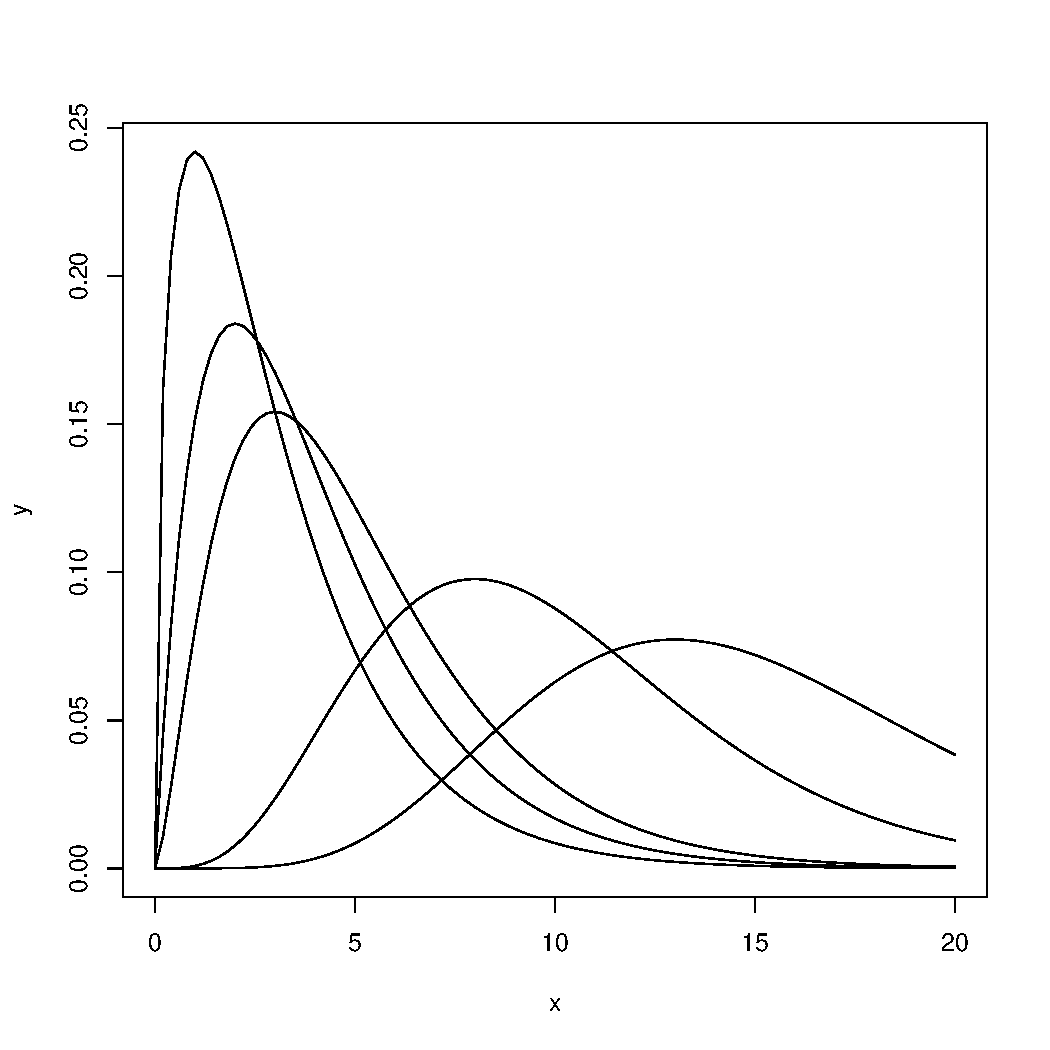
\includegraphics[angle=270, totalheight=4in]{ps/contdist/chisq-dist-vary-df.ps}
  \caption[Chi square distribution for various degrees of freedom]{\small The chi square distribution for various degrees of freedom.}
  \label{fig-chisq-dist-vary-df}
\end{figure}


\begin{rem}
Here are some useful things to know about the chi-square distribution.
\begin{enumerate}
\item If \(Z\sim\mathtt{norm}(\mathtt{mean}=0,\,\mathtt{sd}=1)\), then \(Z^{2}\sim\mathsf{chisq}(\mathtt{df}=1)\). We saw this in Example \ref{exa-distn-of-z-squared}, and the fact is important when it comes time to find the distribution of the sample variance, \(S^{2}\). See Theorem \ref{thm-Xbar-and-S} in Section \ref{sub-Samp-Var-Dist}.
\item The chi-square distribution is supported on the positive \(x\)-axis, with a right-skewed distribution.
\item The \(\mathsf{chisq}(\mathtt{df}=p)\) distribution is the same as a \(\mathsf{gamma}(\mathtt{shape}=p/2,\,\mathtt{rate}=1/2)\) distribution.
\item The MGF of \(X\sim\mathsf{chisq}(\mathtt{df}=p)\) is
   \begin{equation}
   M_{X}(t)=\left(1-2t\right)^{-p},\quad t<1/2.\label{eq-mgf-chisq}
   \end{equation}
\end{enumerate}

\end{rem}
\subsubsection{Student's \(t\) distribution}
\label{sec-1-5-2-2}
\label{sub-Student's-t-distribution}


A random variable \(X\) with PDF
\begin{equation}
f_{X}(x) = \frac{\Gamma\left[ (r+1)/2\right] }{\sqrt{r\pi}\,\Gamma(r/2)}\left( 1 + \frac{x^{2}}{r} \right)^{-(r+1)/2},\quad -\infty < x < \infty
\end{equation}
is said to have \emph{Student's} \(t\) distribution with \(r\) \emph{degrees of freedom}, and we write \(X\sim\mathsf{t}(\mathtt{df}=r)\). The associated \(\mathsf{R}\) functions are \texttt{dt},=pt=, \texttt{qt}, and \texttt{rt}, which give the PDF, CDF, quantile function, and simulate random variates, respectively. See Section \ref{sec-sampling-from-normal-dist}.
\subsubsection{Snedecor's \(F\) distribution}
\label{sec-1-5-2-3}
\label{sub-snedecor-F-distribution}


A random variable \(X\) with PDF
\begin{equation}
f_{X}(x)=\frac{\Gamma[(m+n)/2]}{\Gamma(m/2)\Gamma(n/2)}\left(\frac{m}{n}\right)^{m/2}x^{m/2-1}\left(1+\frac{m}{n}x\right)^{-(m+n)/2},\quad x>0.
\end{equation}
is said to have an \(F\) distribution with \((m,n)\) degrees of freedom. We write \(X\sim\mathsf{f}(\mathtt{df1}=m,\,\mathtt{df2}=n)\). The associated \(\mathsf{R}\) functions are \texttt{df(x, df1, df2)}, \texttt{pf}, \texttt{qf}, and \texttt{rf}, which give the PDF, CDF, quantile function, and simulate random variates, respectively. We define \(F_{\alpha}(m,n)\) as the number on the \(x\)-axis such that there is exactly \(\alpha\) area under the \(\mathsf{f}(\mathtt{df1}=m,\,\mathtt{df2}=n)\) curve to its right. 

\begin{rem}
Here are some notes about the \(F\) distribution.
\begin{enumerate}
\item If \(X\sim\mathsf{f}(\mathtt{df1}=m,\,\mathtt{df2}=n)\) and \(Y=1/X\), then \(Y\sim\mathsf{f}(\mathtt{df1}=n,\,\mathtt{df2}=m)\). Historically, this fact was especially convenient. In the old days, statisticians used printed tables for their statistical calculations. Since the \(F\) tables were symmetric in \(m\) and \(n\), it meant that publishers could cut the size of their printed tables in half. It plays less of a role today now that personal computers are widespread.
\item If \(X\sim\mathsf{t}(\mathtt{df}=r)\), then \(X^{2}\sim\mathsf{f}(\mathtt{df1}=1,\,\mathtt{df2}=r)\). We will see this again in Section \ref{sub-slr-overall-F-statistic}.
\end{enumerate}

\end{rem}
\subsection{Other Popular Distributions}
\label{sec-1-5-3}
\label{sub-Other-Popular-Distributions}
\subsubsection{The Cauchy Distribution}
\label{sec-1-5-3-1}
\label{sub-The-Cauchy-Distribution}


This is a special case of the Student's \(t\) distribution. It has PDF
\begin{equation}
f_{X}(x) = \frac{1}{\beta\pi} \left[ 1+\left( \frac{x-m}{\beta} \right)^{2} \right]^{-1},\quad -\infty < x < \infty.
\end{equation}
We write \(X\sim\mathsf{cauchy}(\mathtt{location}=m,\,\mathtt{scale}=\beta)\). The associated \(\mathsf{R}\) function is \texttt{dcauchy(x, location = 0, scale = 1)}.

It is easy to see that a \(\mathsf{cauchy}(\mathtt{location}=0,\,\mathtt{scale}=1)\) distribution is the same as a \(\mathsf{t}(\mathtt{df}=1)\) distribution. The \(\mathsf{cauchy}\) distribution looks like a \(\mathsf{norm}\) distribution but with very heavy tails. The mean (and variance) do not exist, that is, they are infinite. The median is represented by the \(\mathtt{location}\) parameter, and the \(\mathtt{scale}\) parameter influences the spread of the distribution about its median.
\subsubsection{The Beta Distribution}
\label{sec-1-5-3-2}
\label{sub-The-Beta-Distribution}


This is a generalization of the continuous uniform distribution.
\begin{equation}
f_{X}(x)=\frac{\Gamma(\alpha+\beta)}{\Gamma(\alpha)\Gamma(\beta)}\, x^{\alpha-1}(1-x)^{\beta-1},\quad 0 < x < 1.
\end{equation}
We write \(X\sim\mathsf{beta}(\mathtt{shape1}=\alpha,\,\mathtt{shape2}=\beta)\). The associated \(\mathsf{R}\) function is \texttt{dbeta(x, shape1, shape2)}. The mean and variance are
\begin{equation} 
\mu=\frac{\alpha}{\alpha+\beta}\mbox{ and }\sigma^{2}=\frac{\alpha\beta}{\left(\alpha+\beta\right)^{2}\left(\alpha+\beta+1\right)}.
\end{equation}
See Example \ref{exa-cont-pdf3x2}. This distribution comes up a lot in Bayesian statistics because it is a good model for one's prior beliefs about a population proportion \(p\), \(0\leq p\leq1\).
\subsubsection{The Logistic Distribution}
\label{sec-1-5-3-3}
\label{sub-The-Logistic-Distribution}


\begin{equation}
f_{X}(x)=\frac{1}{\sigma}\exp\left(-\frac{x-\mu}{\sigma}\right)\left[1+\exp\left(-\frac{x-\mu}{\sigma}\right)\right]^{-2},\quad -\infty < x < \infty.
\end{equation}
We write \(X\sim\mathsf{logis}(\mathtt{location}=\mu,\,\mathtt{scale}=\sigma)\). The associated \(\mathsf{R}\) function is \texttt{dlogis(x, location = 0, scale = 1)}. The logistic distribution comes up in differential equations as a model for population growth under certain assumptions. The mean is \(\mu\) and the variance is \(\pi^{2}\sigma^{2}/3\).
\subsubsection{The Lognormal Distribution}
\label{sec-1-5-3-4}
\label{sub-The-Lognormal-Distribution}


This is a distribution derived from the normal distribution (hence the name). If \(U\sim\mathtt{norm}(\mathtt{mean}=\mu,\,\mathtt{sd}=\sigma)\), then \( X = \mathrm{e}^{U} \) has PDF
\begin{equation}
f_{X}(x)=\frac{1}{\sigma x\sqrt{2\pi}}\exp\left[\frac{-(\ln x-\mu)^{2}}{2\sigma^{2}}\right], \quad 0 < x < \infty.
\end{equation}
We write \(X\sim\mathsf{lnorm}(\mathtt{meanlog}=\mu,\,\mathtt{sdlog}=\sigma)\). The associated \(\mathsf{R}\) function is \texttt{dlnorm(x, meanlog = 0, sdlog = 1)}. Notice that the support is concentrated on the positive \(x\) axis; the distribution is right-skewed with a heavy tail. See Example \ref{exa-lnorm-transformation}.
\subsubsection{The Weibull Distribution}
\label{sec-1-5-3-5}
\label{sub-The-Weibull-Distribution}


This has PDF
\begin{equation}
f_{X}(x)=\frac{\alpha}{\beta}\left(\frac{x}{\beta}\right)^{\alpha-1}\exp\left(\frac{x}{\beta}\right)^{\alpha},\quad x>0.
\end{equation}
We write \(X\sim\mathsf{weibull}(\mathtt{shape}=\alpha,\,\mathtt{scale}=\beta)\). The associated \(\mathsf{R}\) function is \texttt{dweibull(x, shape, scale = 1)}. 
\subsubsection{How to do it with \(\mathsf{R}\)}
\label{sec-1-5-3-6}


There is some support of moments and moment generating functions for some continuous probability distributions included in the \texttt{actuar} package \cite{Dutangactuar}. The convention is \texttt{m} in front of the distribution name for raw moments, and \texttt{mgf} in front of the distribution name for the moment generating function. At the time of this writing, the following distributions are supported: gamma, inverse Gaussian, (non-central) chi-squared, exponential, and uniform.

\begin{example}
Calculate the first four raw moments for \(X\sim\mathsf{gamma}(\mathtt{shape}=13,\,\mathtt{rate}=1)\) and plot the moment generating function.

We load the \texttt{actuar} package and use the functions \texttt{mgamma} and \texttt{mgfgamma}:

\lstset{language=R}
\begin{lstlisting}
library(actuar)
mgamma(1:4, shape = 13, rate = 1)
\end{lstlisting}

\begin{verbatim}
 [1]    13   182  2730 43680
\end{verbatim}

For the plot we can use the function in the following form:


\lstset{language=R}
\begin{lstlisting}
plot(function(x){mgfgamma(x, shape = 13, rate = 1)}, from=-0.1, to=0.1, ylab = "gamma mgf")
\end{lstlisting}





\begin{figure}[th]
  \includegraphics[angle=270, totalheight=4in]{ps/contdist/gamma-mgf.ps}
  \caption[Plot of the \textsf{gamma}(\texttt{shape} = 13, \texttt{rate} = 1) MGF]{\small A plot of the \textsf{gamma}(\texttt{shape} = 13, \texttt{rate} = 1) MGF.}
  \label{fig-gamma-mgf}
\end{figure}


\end{example}

\newpage{}
\section{Exercises}
\label{sec-1-6}

\setcounter{thm}{0}

\begin{xca}
Find the constant \(c\) so that the given function is a valid PDF of a random variable \(X\).
\begin{enumerate}
\item \( f(x) = Cx^{n},\quad 0 < x <1 \).
\item \( f(x) = Cx\mathrm{e}^{-x},\quad 0 < x < \infty\).
\item \( f(x) = \mathrm{e}^{-(x - C)}, \quad 7 < x < \infty.\)
\item \( f(x) = Cx^{3}(1 - x)^{2},\quad 0 < x < 1.\)
\item \( f(x) = C(1 + x^{2}/4)^{-1}, \quad -\infty < x < \infty.\)
\end{enumerate}

\end{xca}

\begin{xca}
For the following random experiments, decide what the distribution of \(X\) should be. In nearly every case, there are additional assumptions that should be made for the distribution to apply; identify those assumptions (which may or may not strictly hold in practice).
\begin{enumerate}
\item We throw a dart at a dart board. Let \(X\) denote the squared linear distance from the bulls-eye to the where the dart landed.
\item We randomly choose a textbook from the shelf at the bookstore and let \(P\) denote the proportion of the total pages of the book devoted to exercises.
\item We measure the time it takes for the water to completely drain out of the kitchen sink.
\item We randomly sample strangers at the grocery store and ask them how long it will take them to drive home.
\end{enumerate}

\end{xca}

\begin{xca}
If \(Z\) is \(\mathsf{norm}(\mathtt{mean}=0,\,\mathtt{sd}=1)\), find 
\begin{enumerate}
\item \(\mathbb{P}(Z>2.64)\)

\lstset{language=R}
\begin{lstlisting}
   pnorm(2.64, lower.tail = FALSE)
\end{lstlisting}
\end{enumerate}

\begin{enumerate}
\item \(\mathbb{P}(0\leq Z<0.87)\)

\lstset{language=R}
\begin{lstlisting}
   pnorm(0.87) - 1/2
\end{lstlisting}
\end{enumerate}

\begin{enumerate}
\item \(\mathbb{P}(|Z|>1.39)\) (Hint: draw a picture!)

\lstset{language=R}
\begin{lstlisting}
   2 * pnorm(-1.39)
\end{lstlisting}
\end{enumerate}

\end{xca}

\begin{xca}
Calculate the variance of \(X\sim\mathsf{unif}(\mathtt{min}=a,\,\mathtt{max}=b)\). \emph{Hint:} First calculate \(\mathbb{E} X^{2}\).
\end{xca}

\begin{xca}
Prove the memoryless property for exponential random variables. That is, for \(X\sim\mathsf{exp}(\mathtt{rate}=\lambda)\) show that for any \(s,t>0\),
\[
\mathbb{P}(X>s+t\,|\, X>t)=\mathbb{P}(X>s).
\]
\end{xca}

\end{document}